\documentclass[12pt]{article}
\usepackage{graphicx}
\usepackage{color}

\begin{document}
\begin{titlepage}
\begin{center}
\begin{huge}
\begin{center}
\textcolor{blue}{Documentation: V3D Digraph Visualizer}
\end{center}
\end{huge}
\hfill \break
\begin{Large}
\begin{center}
\textcolor{blue}{Team: App-Synth}
\end{center}
\end{Large}
\begin{small}
\begin{flushleft}
Author(s):
\end{flushleft}

\begin{itemize}
  \item Kulani Bamuza \\
  \item Keanan Jones \\
  \item Munyaradzi Mpofu\\
  \item Neo Thokoa\\  
  \item Takalani Sigama\\
  
\end{itemize}
\end{small}

\end{center}
\begin{center}
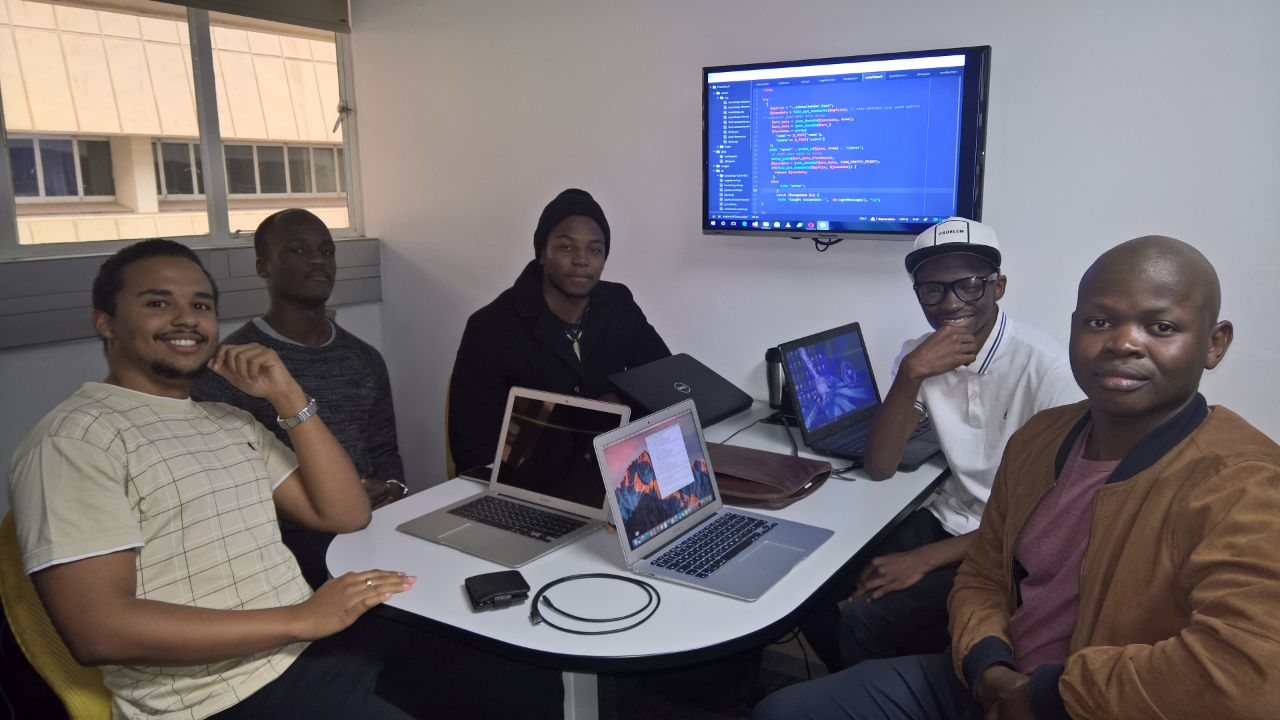
\includegraphics[scale=0.4]{Dps/TeamPic.jpg}
\\
\textcolor{blue}{\textit{University of Pretoria, Department of Computer Science
\\
}}

\end{center}
\end{titlepage}

\newpage
\pagenumbering{arabic}
\thispagestyle{empty}
\tableofcontents
\clearpage

\textcolor{blue}{\section{Introduction}}
\textcolor{blue}{\subsection{Project Background}}
\begin{flushleft}
The V3D Digraph Visualizer is a tool used to visualize digraphs in a 3D virtual reality environment. Users can also interact with the graph. This is done using an on-screen reticle. Possible interactions include moving, adding and removing nodes from the graph. Our app is powered by the Unity game engine and the Google Cardboard SDK
\end{flushleft}

\textcolor{blue}{\subsection{Project Vision}}
\begin{flushleft}
Virtual reality and supporting technologies are relatively new. Their use cases are only recently beginning to see exploration from adopters of the technologies. The V3D Digraph Visualiser is an instance of the use cases of the mentioned technologies. Products such as ours aim to position us among early users of the technologies.
\end{flushleft}

\textcolor{blue}{\subsection{Project Scope}}
\begin{flushleft}
The digraph is stored as a set of triples, as specified by Barla-Szabo. The user, within the virtual environment, should be able to look around and observe the structure of the graph and its components. Information about the graph's data points are also displayed on the screen. This metadata will provide the necessary information required to produce a force directed graph. The users will be immersed in the 3D environment by means of virtual reality 3D glasses. The user may use a VR headset such as Google Cardboard which they are able to build themselves. Besides viewing the graph, the viewer should be able to interact with the graph by manipulating the metadata related to certain vertices and edges. Observers may view the 3D environment on an external display.
\end{flushleft}

\textcolor{blue}{\section{Overall Description}}
\textcolor{blue}{\subsection{Product Perspective}}
\begin{flushleft}
The system is deployed as mobile Android app. The user must have a Google Cardboard headset or similar device. This application will contain a graphical user interface through which the user can make use of the system. The mobile application itself will interact with various components of the mobile device, including the camera and the gyroscope. The scene displayed on the mobile device is also displayed on an external display. 
\end{flushleft}

\textcolor{blue}{\subsection{Product Function}}
\begin{flushleft}
The system also allows a previously created graph to be read into the app. Once the graph has been loaded, it will be visualized in the 3D environment. The graph is also force directed. The user is also able to navigate through the graph. Navigation includes zooming in and out as well as rotating the graph. Navigation is facilitated by on-screen buttons. Interaction with the graph is done using an on-screen reticle. The reticle is set to remain pointed in the direction in which the user is looking. Focusing the reticle on a node for two seconds is functionally similar to picking a node up. A node turns blue once it is "picked up". The user is then able to look in the direction he/she wishes to place the node. The user can "drop" the node by keeping their gaze fixated at a point for two seconds. Changes made to the graph can be saved into a text file The system should allow for observers to view the graph which is being viewed by the user from the user’s perspective and the visuals which the observers see should be updated accordingly as the user’s viewport changes. This is made possible using the TeamViewer app. TeamViewer must be installed on the phone as well as the external device
\end{flushleft}

\textcolor{blue}{\subsection{User Characteristics}}
\begin{flushleft}
The typical user groups of the system can be categorized into two different user groups, namely education professionals (academics, researchers and students) and the "everyday user" (any individual with general graph knowledge). Education professionals may use the graph visualizations to assist with educational activities and the visualizer will also aid researchers in their research activities. For undergraduate students, the graph visualizer will be a useful tool which will assist them in gaining a better understanding of graphs. All of the user groups must have a general understanding of graphs and their various applications. The user must also possess an understanding of certain graph-related concepts such as force direction. The user should possess basic computer literacy skills
\end{flushleft}

\textcolor{blue}{\subsection{Constraints}}
\begin{flushleft}
 The mobile app requires a device running, at minimum, Android 4.1.1 (KitKat). The overall system should be modular to allow for the addition of features as the need arises. Support for other operating systems may be considered in future
\end{flushleft}

\textcolor{blue}{\subsection{Assumptions and Dependencies}}
\begin{flushleft}
The devices on which the system is deployed should contain the necessary hardware which is needed for the system to function. Requirements include a gyroscope and networking capabilities. The user will also need to have access to a pair of virtual reality glasses in order to visualize the graphs in a 3D environment.
\end{flushleft}

\textcolor{blue}{\section{Functional Product Requirements}}
\begin{flushleft}
  
  \textcolor{blue}{\subsection{Creation Module}}  
  \begin{flushleft}
  \begin{itemize}
  \item CRUD graph
  \end{itemize} 
  \end{flushleft}
  
  \textcolor{blue}{\subsection{Control Module}} 
  \begin{flushleft}
  \begin{itemize}
  \item Facilitate user interaction with the graph through the on-screen reticle
  \item Provide button functionality to allow switching scenes
  \end{itemize} 
  \end{flushleft}
  
  \textcolor{blue}{\subsection{Rendering Module}} 
  \begin{flushleft}
  \begin{itemize}
  \item Take formatted graph information and construct a graph
  \item Provide real time rendering from user interactions
  \item Render graph to external display
  \end{itemize} 
  \end{flushleft}
  
  \textcolor{blue}{\subsection{Serialisation Module}} 
  \begin{flushleft}
  \begin{itemize}
  \item Convert graph text file into JSON object
  \item Save state of graph as JSON object
  \end{itemize} 
  \end{flushleft}

\end{flushleft}

\textcolor{blue}{\section{Non-functional Product Requirements}}
\begin{flushleft}
The system should be able to respond to user actions in a timely manner to allow for smooth user interaction. This requirement is especially vital for user interactions with the graph visualization. There should be real time communication between the mobile application and the desktop application to allow observers to witness the user’s interactions with the graph in real time.

\bigskip

\textcolor{blue}{\subsection{Extensibility}}
The system must be robust and modular, allowing for simple alterations to the current system and to cater for the future growth of the system by allowing additional features to be implemented and incorporated with ease.

\bigskip

\textcolor{blue}{\subsection{Reliability}}
The system should be able to process user input accurately and respond appropriately at all times.

\bigskip

\textcolor{blue}{\subsection{Usability}}
The system should be user friendly. 

\end{flushleft}

\textcolor{blue}{\section{Use Cases}}
\textcolor{blue}{\subsection{Control Module}}

\begin{flushleft}
UC1.1 Select Vertex
\begin{itemize}
\item[i] Description: User selects node by focusing pointer at it 
\item[ii] Pre-condition: The user must be viewing the graph in a 3D environment.
\item[iii] Post-condition: The desired node changes colour and is movable 
\end{itemize}
\end{flushleft}

\begin{flushleft}
UC1.2 Open URL
\begin{itemize}
\item[i] Description: User navigates from app to web browser and opens graph creation web interface
\item[ii] Pre-condition: Menu is displayed on screen
\item[iii] Post-condition: Webpage is displayed on the screen
\end{itemize}
\end{flushleft}

\bigskip

\begin{flushleft}
UC1.3 Open file selector
\begin{itemize}
\item[i] Description: User navigates from app to file selector to open existing graph
\item[ii] Pre-condition: Menu is displayed on screen
\item[iii] Post-condition: File selector interface is displayed on the screen
\end{itemize}
\end{flushleft}

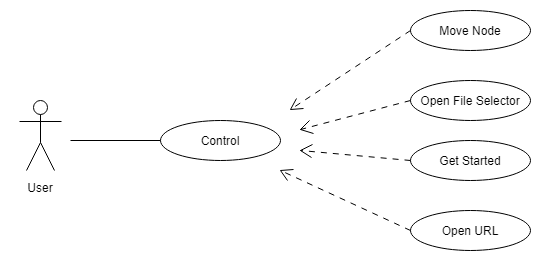
\includegraphics[scale=0.5]{Dps/Control.png}

\bigskip

\textcolor{blue}{\subsection{Creation Module}}
\begin{flushleft}
UC2.1 Create Node
\begin{itemize}
\item[i] Description: The system should allow for the user to create a new vertex and add it to the graph visualization.
\item[ii] Pre-condition: The user must be viewing the graph in a 3D environment.
\item[iii] Post-condition: A vertex has been added to the graph.
\end{itemize}
\end{flushleft}

\bigskip

\begin{flushleft}
UC2.2 Update Graph
\begin{itemize}
\item[i] Description: The system should allow for the user to update data within the graph
\item[ii] Pre-condition: Graph file contents must be open
\item[iii] Post-condition: Contents updated and saved.
\end{itemize}
\end{flushleft}

\bigskip

\begin{flushleft}
UC2.3 Remove Node
\begin{itemize}
\item[i] Description: The system should allow for the user to remove a node from the graph visualization.
\item[ii] Pre-condition: User must be viewing the graph in a 3D environment.
\item[iii] Post-condition: A vertex has been removed from the graph.
\end{itemize}
\end{flushleft}
\bigskip


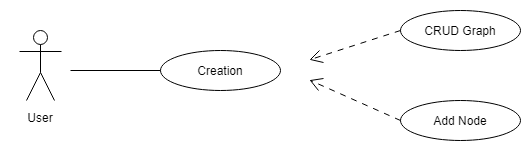
\includegraphics[scale=0.5]{Dps/Creation.png}

\textcolor{blue}{\subsection{Rendering Module}}

\begin{flushleft}
UC3.1 Render Graph on External Display
\begin{itemize}
\item[i] Description: Mirror mobile display on external display
\item[ii] Pre-condition: Connection to external display must be set up
\item[iii] Post-condition: Graph is rendered and displays are synchronised
\end{itemize}
\end{flushleft}

\bigskip

\begin{flushleft}
UC3.2 Render VR Graph
\begin{itemize}
\item[i]Description: Create graph from JSON representation
\item[ii] Pre-condition: Graph has been loaded from text file into data structure
\item[iii] Post-condition: A graph has been rendered on the external display.
\end{itemize}
\end{flushleft}

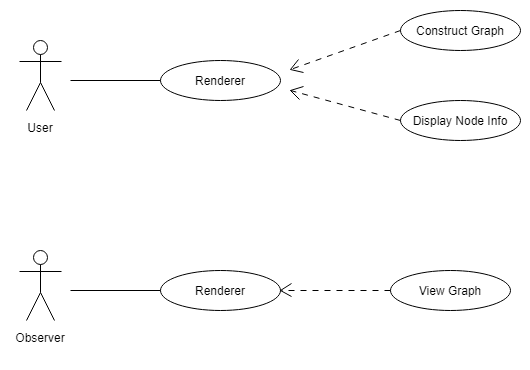
\includegraphics[scale=0.5]{Dps/Renderer}

\textcolor{blue}{\subsection{Serialization Module}}
\begin{flushleft}
UC4.1 Load Graph File
\begin{itemize}
\item[i] Description: Read text file and convert contents into JSON object for display
\item[ii] Pre-condition: Graph text file must be present on device
\item[iii] Post-condition: Variable containing graph is set
\end{itemize}
\end{flushleft}

\begin{flushleft}
UC4.2 Serialize
\begin{itemize}
\item[i]Description: The app should convert state of the graph into JSON object
\item[ii] Pre-condition: Graph must be loaded
\item[iii] Post-condition: Variable containing JSON data is set
\end{itemize}
\end{flushleft}

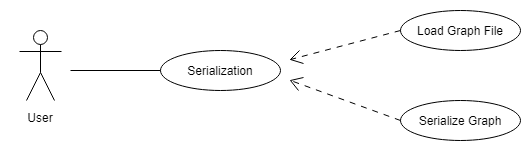
\includegraphics[scale=0.5]{Dps/Serialization}


\end{document}